\documentclass[
	a4paper,
	oneside,
	BCOR = 10mm,
	DIV = 12,
	12pt,
	headings = normal,
]{scrartcl}

%%% Length calculations
\usepackage{calc}
%%%

%%% Support for color
\usepackage{xcolor}
\definecolor{lightblue}{HTML}{03A9F4}
\definecolor{red}{HTML}{F44336}
%%%

%%% Including graphics
\usepackage{graphicx}
%%%

%%% Font selection
\usepackage{fontspec}

\setromanfont{STIX Two Text}[
	SmallCapsFeatures = {LetterSpace = 8},
]

\setsansfont{IBM Plex Sans}[
	Scale = MatchUppercase,
]

\setmonofont{IBM Plex Mono}[
	Scale = MatchUppercase,
]
%%%

%%% Math typesetting
\usepackage{amsmath}

\usepackage{unicode-math}
\setmathfont{STIX Two Math}
%%%

%%% List settings
\usepackage{enumitem}
\setlist[enumerate]{
	label*      = {\arabic*.},
	leftmargin  = *,
	labelindent = \parindent,
	topsep      = 1\baselineskip,
	parsep      = 0\baselineskip,
	itemsep     = 1\baselineskip,
}

\setlist[itemize]{
	label*      = {—},
	leftmargin  = *,
	labelindent = \parindent,
	topsep      = 1\baselineskip,
	parsep      = 0\baselineskip,
	itemsep     = 1\baselineskip,
}

\setlist[description]{
	font        = {\rmfamily\upshape\bfseries},
	topsep      = 1\baselineskip,
	parsep      = 0\baselineskip,
	itemsep     = 0\baselineskip,
}

%%%

%%% Structural elements typesetting
\setkomafont{pagenumber}{\rmfamily}
\setkomafont{disposition}{\rmfamily\bfseries}

% Sectioning
\RedeclareSectionCommand[
	beforeskip = -1\baselineskip,
	afterskip  = 1\baselineskip,
	font       = {\normalsize\bfseries\scshape},
]{section}

\RedeclareSectionCommand[
	beforeskip = -1\baselineskip,
	afterskip  = 1\baselineskip,
	font       = {\normalsize\bfseries\itshape},
]{subsection}

\RedeclareSectionCommand[
	beforeskip = -1\baselineskip,
	afterskip  = 1\baselineskip,
	font       = {\normalsize\bfseries},
]{subsubsection}

\RedeclareSectionCommand[
	beforeskip = -1\baselineskip,
	afterskip  = -0.5em,
	font       = {\normalsize\mdseries\scshape\addfontfeatures{Letters = {UppercaseSmallCaps}}},
]{paragraph}
%%%

%%% Typographic enhancements
\usepackage{microtype}
%%%

%%% Language-specific settings
\usepackage{polyglossia}
\setmainlanguage{ukrainian}
\setotherlanguages{english}
%%%

%%% Captions
\usepackage{caption}
\usepackage{subcaption}

%\DeclareCaptionLabelFormat{closing}{#2)}
%\captionsetup[subtable]{labelformat = closing}

%\captionsetup[subfigure]{labelformat = closing}

\captionsetup[table]{
	aboveskip = 0\baselineskip,
	belowskip = 0\baselineskip,
}

\captionsetup[figure]{
	aboveskip = 1\baselineskip,
	belowskip = 0\baselineskip,
}

\captionsetup[subfigure]{
	labelformat = simple,
	labelformat = brace,
}
%%%

%%% Hyphenated ragged typesetting
\usepackage{ragged2e}
%%%

%%% Table typesetting
\usepackage{booktabs}
\usepackage{longtable}

\usepackage{multirow}

\usepackage{array}
\newcolumntype{v}[1]{>{\RaggedRight\arraybackslash\hspace{0pt}}p{#1}}
\newcolumntype{b}[1]{>{\Centering\arraybackslash\hspace{0pt}}p{#1}}
\newcolumntype{n}[1]{>{\RaggedLeft\arraybackslash\hspace{0pt}}p{#1}}
%%%

%%% Drawing
\usepackage{tikz}
\usepackage{tikzscale}
\usetikzlibrary{positioning}
\usetikzlibrary{arrows.meta} % Stealth arrow tips
%%%

%%% SI units typesetting
\usepackage{siunitx}
\sisetup{
	output-decimal-marker = {,},
	exponent-product      = {\cdot},
	inter-unit-product    = \ensuremath{{} \cdot {}},
	per-mode              = symbol,
}
%%%

%%% Links and hyperreferences
\usepackage{hyperref}
\hypersetup{
	bookmarksnumbered = true,
	colorlinks      = false,
	linkbordercolor = red,
	urlbordercolor  = lightblue,
	pdfborderstyle  = {/S/U/W 1.5},
}
%%%

%%% Length adjustments
% Set baselineskip, default is 14.5 pt
\linespread{1.068966} % ~15.5 pt
\setlength{\emergencystretch}{1em}
\setlength{\parindent}{1.5em}
\newlength{\gridunitwidth}
\setlength{\gridunitwidth}{\textwidth / 12}
%%%

%%% Boldface math in sectioning commands
\makeatletter
\g@addto@macro\bfseries{\boldmath}
\makeatother
%%%

%%% Custom commands
\newcommand{\allcaps}[1]{{\addfontfeatures{LetterSpace = 8, Kerning = Off}#1}}
%%%

\begin{document}

\begin{titlepage}
		\begin{center}
			Міністерство освіти і науки України\\
			Національний авіаційний університет\\
			Навчально-науковий інститут комп'ютерних інформаційних технологій\\
			Кафедра комп'ютеризованих систем управління

			\vspace{\fill}
				Лабораторна робота №2.2\\
				з дисципліни «Телекомунікаційні~технології комп'ютерних~мереж»\\
				на тему «Моделювання каналу зв'язку»

			\vspace{\fill}

			\begin{flushright}
				Виконав:\\
				студент \allcaps{ННІКІТ}\\
				групи СП-325\\
				Клокун В.\,Д.\\
				Перевірив:\\
				Пушкін Ю.\,О.
			\end{flushright}

			Київ 2018
		\end{center}
	\end{titlepage}

	\section{Мета роботи}
		Дослідження явищ, що виникають в каналі зв'язку системи передачі цифрової інформації.

	\section{Завдання роботи}
		Опис теоретичних моделей процесів, що відбуваються в каналі зв'язку; моделювання каналу зв'язку в~\textenglish{Simulink}.

	\section{Хід роботи}
		\subsection{Створення моделі}
			Створюємо модель передавальної системи, яка~складається з~генератора випадкових цілих чисел, модулятора, каналу передачі, спектрального аналізатора, блоку виділення дійсної і~комплексної частин сигналу та~осцилографа~(рис.~\ref{subfig:01-simulink-tx-model-full}).

			\begin{figure}[!htbp]
				\begin{subfigure}[t]{\textwidth / 2}
					\centering
					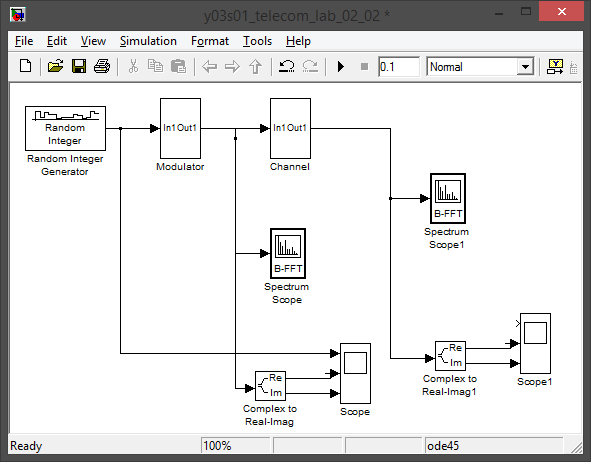
\includegraphics[height = 9\baselineskip]{./assets/y03s01-telecom-lab-02-02-p01-model-general.png}
					\caption{}
					\label{subfig:01-simulink-tx-model-full}
				\end{subfigure}%
				\begin{subfigure}[t]{\textwidth / 2}
					\centering
					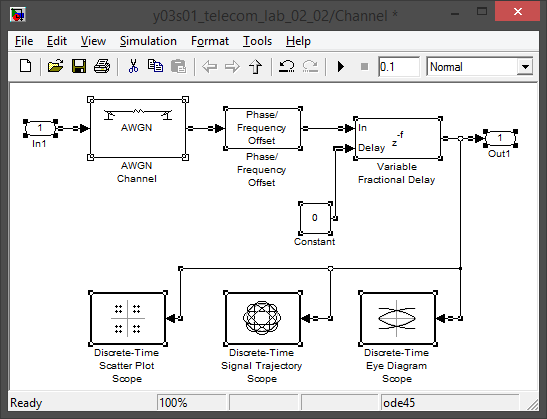
\includegraphics[height = 9\baselineskip]{./assets/y03s01-telecom-lab-02-02-p02-model-channel.png}
					\caption{}
					\label{subfig:01-simulink-tx-model-transmitter}
				\end{subfigure}
				\caption{Модель передавальної системи: \subref{subfig:01-simulink-tx-model-full}~— загальний вигляд, \subref{subfig:01-simulink-tx-model-transmitter}~— канал передачі}
				\label{fig:01-simulink-tx-model}
			\end{figure}

			В~моделі створюємо підсистему каналу передачі, який складається з~генератора адитивного Гаусового шуму, блоку здійснення фазового і частотного зсувів та блоку дробової затримки сигналу~(рис.~\ref{subfig:01-simulink-tx-model-transmitter}).

		\subsection{Симуляція роботи створеної моделі системи передачі даних}
			Для виконання завдання роботи виконуємо симуляцію з різними значеннями відношення «Сигнал~— шум»~(\SI{0}{\deci\bel}, \SI{100}{\deci\bel}), фазового зсуву~(\SI{0}{\degree}, \SI{45}{\degree}), частотного зсуву~(\SI{0}{\hertz}, \SI{1000}{\hertz}) та дробової затримки~(\SI{0}{\second}, \SI{3}{\second}).

			\clearpage
			\subsubsection{Відношення «Сигнал — Шум»~\SI{0}{\deci\bel}, \SI{100}{\deci\bel}}
				Встановлюємо відношення «Сигнал — Шум»~\SI{0}{\deci\bel}, \SI{100}{\deci\bel} та~запускаємо моделювання, отримаємо результати на~графіках~(рис.~\ref{fig:rolloff-0p0-spectrum-scope}, \ref{fig:rolloff-0p0-scope}, \ref{fig:rolloff-0p0-plots}).

				\begin{figure}[!htbp]
					\begin{minipage}[t]{0.5\textwidth - 0.5em}
						\centering
						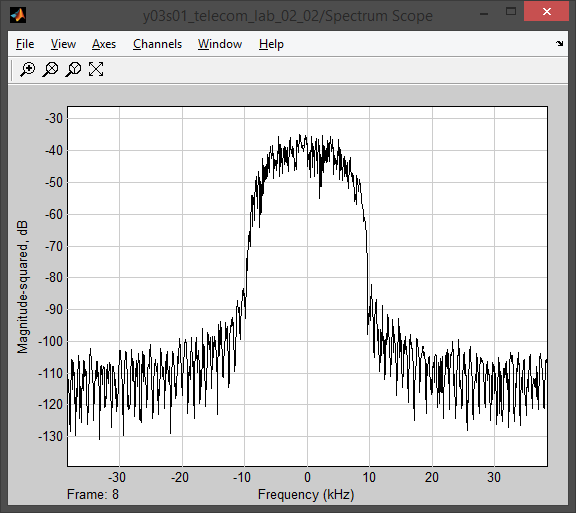
\includegraphics[height = 8\baselineskip]{../01-solution/00-SNR-100db-noshift-modulator-spectrum.png}
						\caption{Спектр сигналу при відношенні «Сигнал — Шум» \SI{100}{\deci\bel}}
						\label{fig:rolloff-0p0-spectrum-scope}
					\end{minipage}\hspace{1em}%
					\begin{minipage}[t]{0.5\textwidth - 0.5em}
						\centering
						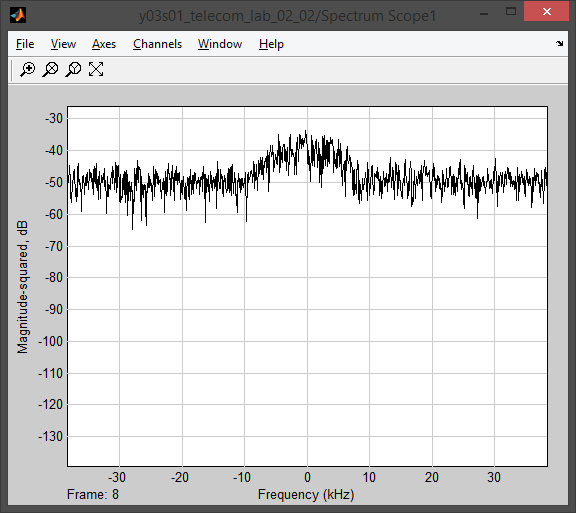
\includegraphics[height = 8\baselineskip]{../01-solution/01-SNR-00-db-channel-spectrum.png}
						\caption{Спектр сигналу при відношенні «Сигнал — Шум» \SI{0}{\deci\bel}}
						\label{fig:rolloff-0p0-scope}
					\end{minipage}%
				\end{figure}

				\begin{figure}[!htbp]
					\centering
					\begin{subfigure}{\textwidth / 3}
						\centering
						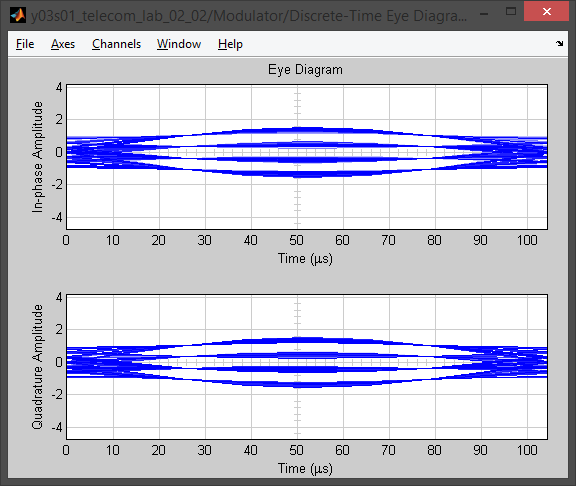
\includegraphics[height = 7\baselineskip]{../01-solution/00-SNR-100db-noshift-modulator-eye-diagram.png}
						\caption{}
						\label{subfig:rolloff-0p0-eye-in}
					\end{subfigure}%
					\begin{subfigure}{\textwidth / 3}
						\centering
						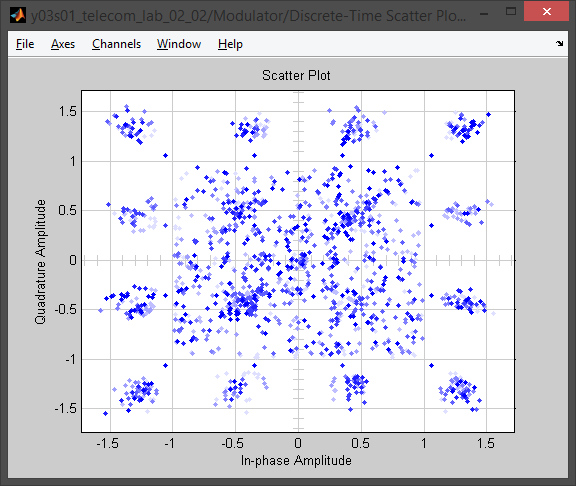
\includegraphics[height = 7\baselineskip]{../01-solution/00-SNR-100db-noshift-modulator-scatter-plot.png}
						\caption{}
						\label{subfig:rolloff-0p0-signal-trajectory-in}
					\end{subfigure}%
					\begin{subfigure}{\textwidth / 3}
						\centering
						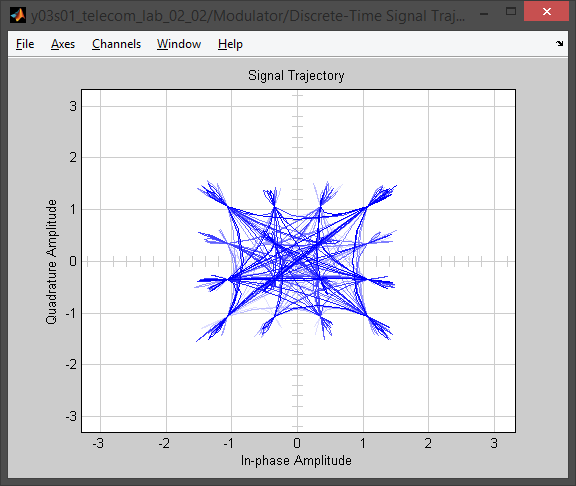
\includegraphics[height = 7\baselineskip]{../01-solution/00-SNR-100db-noshift-modulator-signal-trajectory.png}
						\caption{}
						\label{subfig:rolloff-0p0-scatter-plot-in}
					\end{subfigure}
					\begin{subfigure}{\textwidth / 3}
						\centering
						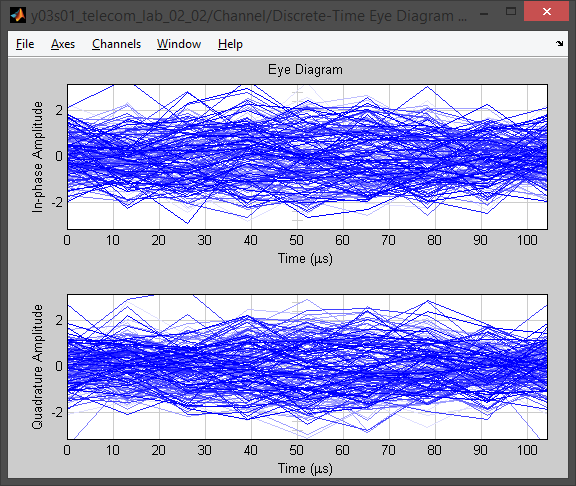
\includegraphics[height = 7\baselineskip]{../01-solution/01-SNR-00-db-channel-eye-diagram.png}
						\caption{}
						\label{subfig:rolloff-0p0-eye-out}
					\end{subfigure}%
					\begin{subfigure}{\textwidth / 3}
						\centering
						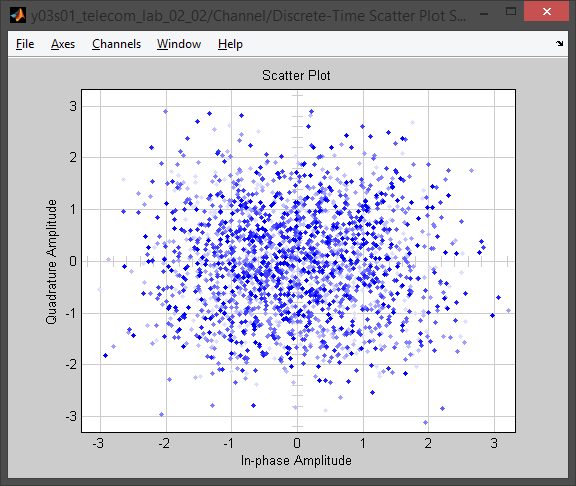
\includegraphics[height = 7\baselineskip]{../01-solution/01-SNR-00-db-channel-scatter-plot.png}
						\caption{}
						\label{subfig:rolloff-0p0-signal-trajectory-out}
					\end{subfigure}%
					\begin{subfigure}{\textwidth / 3}
						\centering
						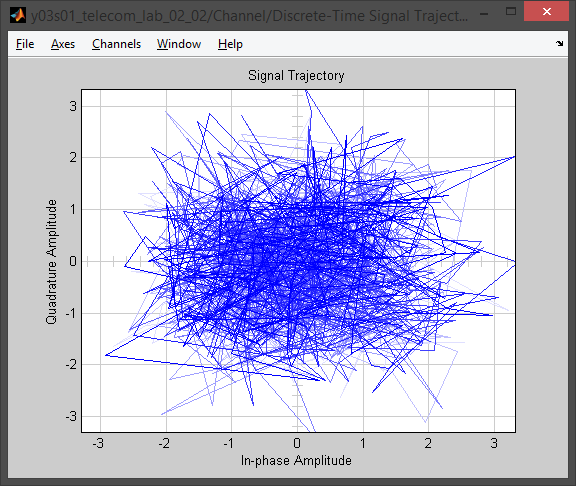
\includegraphics[height = 7\baselineskip]{../01-solution/01-SNR-00-db-channel-signal-trajectory.png}
						\caption{}
						\label{subfig:rolloff-0p0-scatter-plot-out}
					\end{subfigure}%
					\caption{Вплив відношення «Сигнал — Шум» на сигнал: \subref{subfig:rolloff-0p0-eye-in}–\subref{subfig:rolloff-0p0-scatter-plot-in}~— при значенні~\SI{100}{\deci\bel}; \subref{subfig:rolloff-0p0-eye-out}–\subref{subfig:rolloff-0p0-scatter-plot-out}~— при значенні~\SI{0}{\deci\bel}}
					\label{fig:rolloff-0p0-plots}
				\end{figure}

			\subsubsection{Фазова неузгодженість~\SI{0}{\degree}, \SI{45}{\degree}}
				Встановлюємо фазову неузгодженість~\SI{0}{\degree}, \SI{45}{\degree} та~запускаємо моделювання, отримаємо результати на~графіках~(рис.~\ref{fig:phaseshift-spectrum-scope}, \ref{fig:phaseshift-scope}, \ref{fig:phaseshift-plots}).

				\begin{figure}[!htbp]
					\begin{minipage}[t]{0.5\textwidth - 0.5em}
						\centering
						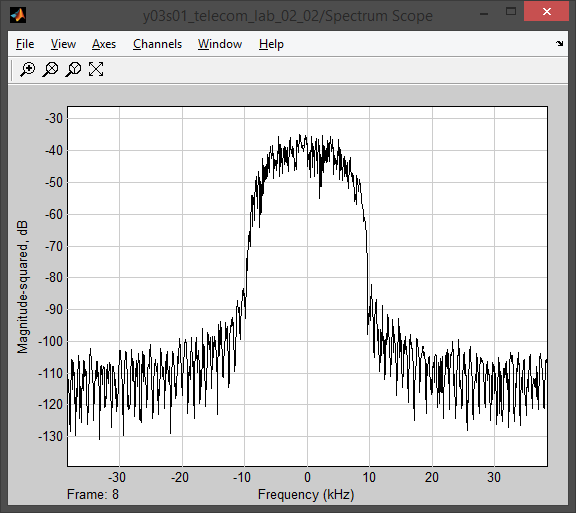
\includegraphics[height = 8\baselineskip]{../01-solution/00-SNR-100db-noshift-modulator-spectrum.png}
						\caption{Спектр сигналу при фазовій неузгодженості \SI{0}{\degree}}
						\label{fig:phaseshift-spectrum-scope}
					\end{minipage}\hspace{1em}%
					\begin{minipage}[t]{0.5\textwidth - 0.5em}
						\centering
						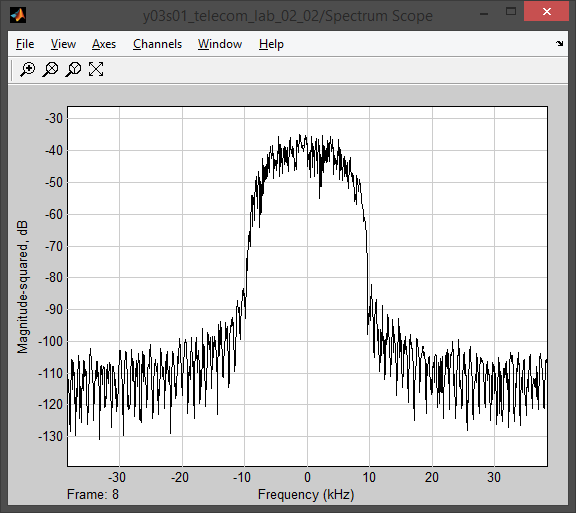
\includegraphics[height = 8\baselineskip]{../01-solution/00-SNR-100db-noshift-modulator-spectrum.png}
						\caption{Спектр сигналу при фазовій неузгодженості \SI{45}{\degree}}
						\label{fig:phaseshift-scope}
					\end{minipage}%
				\end{figure}

				\begin{figure}[!htbp]
					\centering
					\begin{subfigure}{\textwidth / 3}
						\centering
						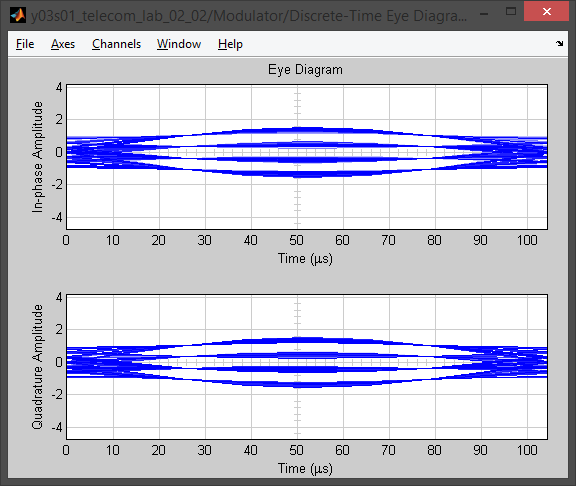
\includegraphics[height = 7\baselineskip]{../01-solution/00-SNR-100db-noshift-modulator-eye-diagram.png}
						\caption{}
						\label{subfig:phaseshift-eye-in}
					\end{subfigure}%
					\begin{subfigure}{\textwidth / 3}
						\centering
						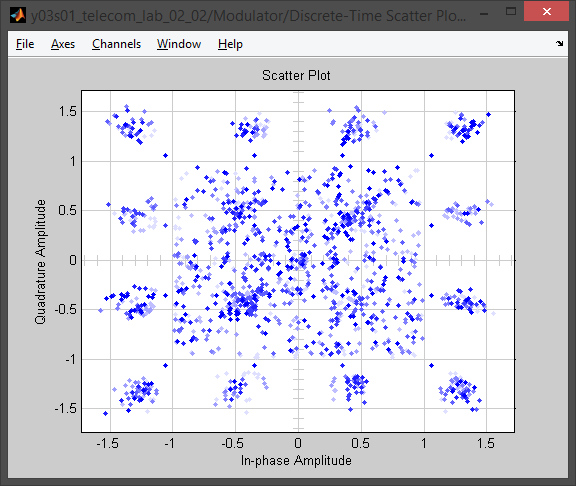
\includegraphics[height = 7\baselineskip]{../01-solution/00-SNR-100db-noshift-modulator-scatter-plot.png}
						\caption{}
						\label{subfig:phaseshift-signal-trajectory-in}
					\end{subfigure}%
					\begin{subfigure}{\textwidth / 3}
						\centering
						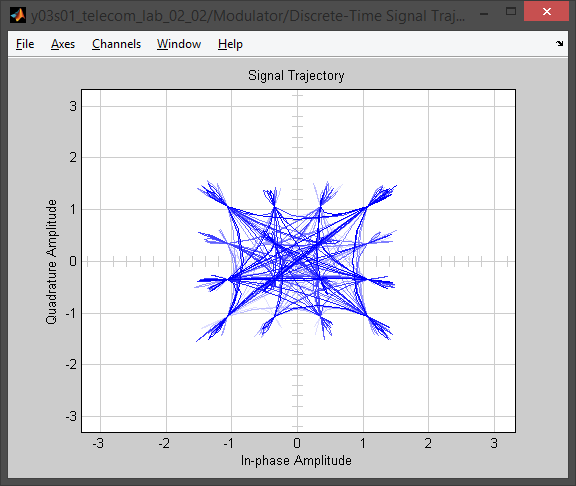
\includegraphics[height = 7\baselineskip]{../01-solution/00-SNR-100db-noshift-modulator-signal-trajectory.png}
						\caption{}
						\label{subfig:phaseshift-scatter-plot-in}
					\end{subfigure}
					\begin{subfigure}{\textwidth / 3}
						\centering
						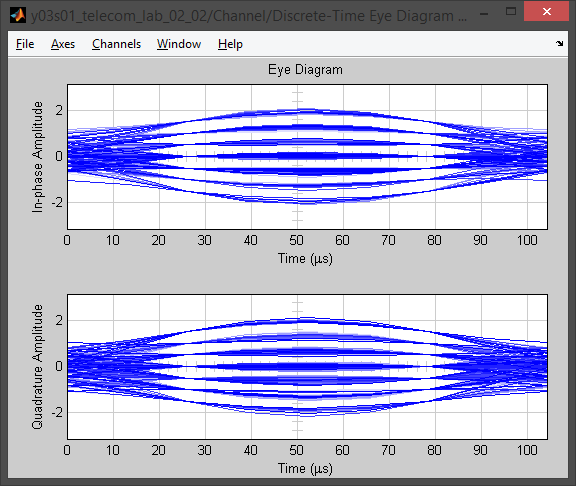
\includegraphics[height = 7\baselineskip]{../01-solution/02-phaseshift-45-deg-channel-eye-diagram.png}
						\caption{}
						\label{subfig:phaseshift-eye-out}
					\end{subfigure}%
					\begin{subfigure}{\textwidth / 3}
						\centering
						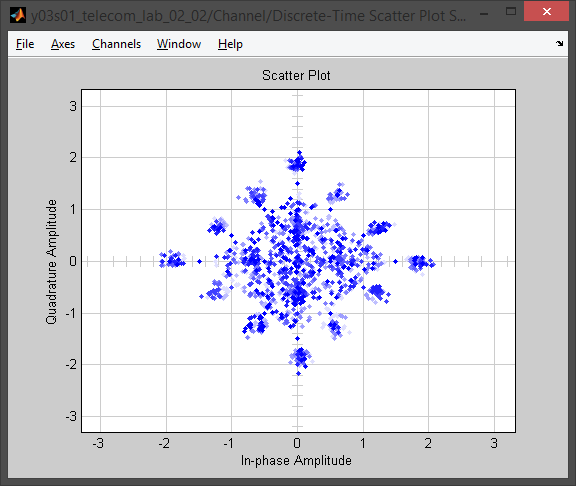
\includegraphics[height = 7\baselineskip]{../01-solution/02-phaseshift-45-deg-channel-scatter-plot.png}
						\caption{}
						\label{subfig:phaseshift-signal-trajectory-out}
					\end{subfigure}%
					\begin{subfigure}{\textwidth / 3}
						\centering
						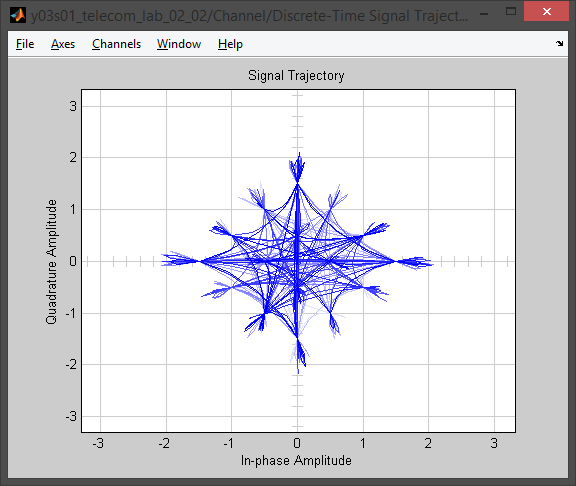
\includegraphics[height = 7\baselineskip]{../01-solution/02-phaseshift-45-deg-channel-signal-trajectory.png}
						\caption{}
						\label{subfig:phaseshift-scatter-plot-out}
					\end{subfigure}%
					\caption{Вплив фазової неузгодженості на сигнал: \subref{subfig:phaseshift-eye-in}–\subref{subfig:phaseshift-scatter-plot-in}~— при значенні~\SI{0}{\degree}; \subref{subfig:phaseshift-eye-out}–\subref{subfig:phaseshift-scatter-plot-out}~— при значенні~\SI{45}{\degree}}
					\label{fig:phaseshift-plots}
				\end{figure}

			\subsubsection{Частотна неузгодженість~\SI{0}{\hertz}, \SI{1000}{\hertz}}
				Встановлюємо частотну неузгодженість~\SI{0}{\hertz}, \SI{1000}{\hertz} та~запускаємо моделювання, отримаємо результати на~графіках~(рис.~\ref{fig:freqshift-spectrum-scope}, \ref{fig:freqshift-scope}, \ref{fig:freqshift-plots}).

				\begin{figure}[!htbp]
					\begin{minipage}[t]{0.5\textwidth - 0.5em}
						\centering
						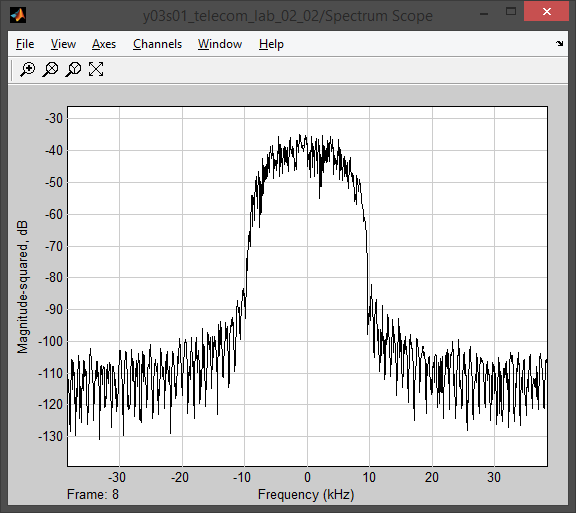
\includegraphics[height = 8\baselineskip]{../01-solution/00-SNR-100db-noshift-modulator-spectrum.png}
						\caption{Спектр сигналу при частотній неузгодженості \SI{0}{\hertz}}
						\label{fig:freqshift-spectrum-scope}
					\end{minipage}\hspace{1em}%
					\begin{minipage}[t]{0.5\textwidth - 0.5em}
						\centering
						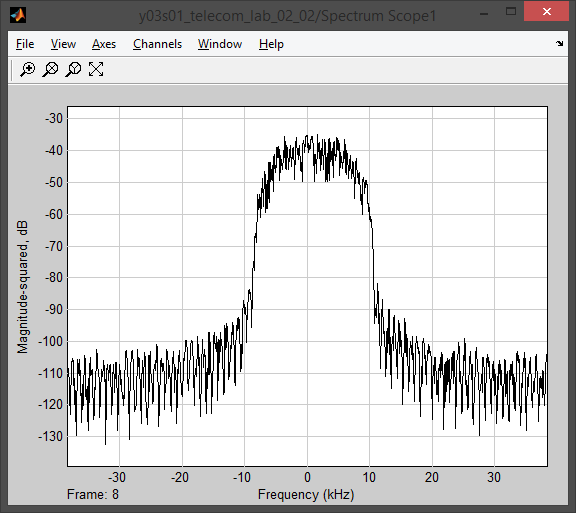
\includegraphics[height = 8\baselineskip]{../01-solution/02-freqshift-1000-hz-channel-spectrum.png}
						\caption{Спектр сигналу при частотній неузгодженості \SI{1000}{\hertz}}
						\label{fig:freqshift-scope}
					\end{minipage}%
				\end{figure}

				\begin{figure}[!htbp]
					\centering
					\begin{subfigure}{\textwidth / 3}
						\centering
						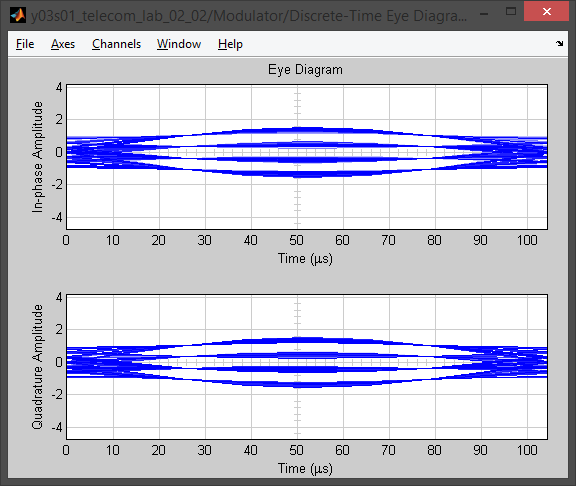
\includegraphics[height = 7\baselineskip]{../01-solution/00-SNR-100db-noshift-modulator-eye-diagram.png}
						\caption{}
						\label{subfig:freqshift-eye-in}
					\end{subfigure}%
					\begin{subfigure}{\textwidth / 3}
						\centering
						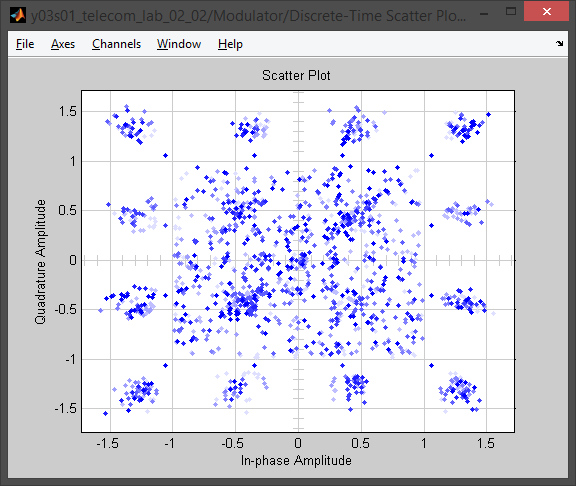
\includegraphics[height = 7\baselineskip]{../01-solution/00-SNR-100db-noshift-modulator-scatter-plot.png}
						\caption{}
						\label{subfig:freqshift-signal-trajectory-in}
					\end{subfigure}%
					\begin{subfigure}{\textwidth / 3}
						\centering
						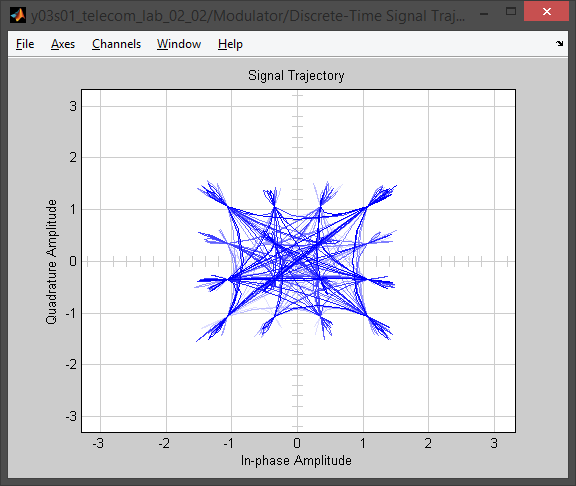
\includegraphics[height = 7\baselineskip]{../01-solution/00-SNR-100db-noshift-modulator-signal-trajectory.png}
						\caption{}
						\label{subfig:freqshift-scatter-plot-in}
					\end{subfigure}
					\begin{subfigure}{\textwidth / 3}
						\centering
						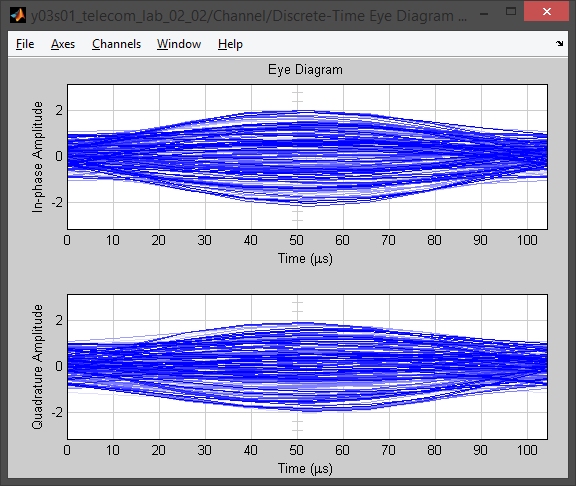
\includegraphics[height = 7\baselineskip]{../01-solution/02-freqshift-1000-hz-channel-eye-diagram.png}
						\caption{}
						\label{subfig:freqshift-eye-out}
					\end{subfigure}%
					\begin{subfigure}{\textwidth / 3}
						\centering
						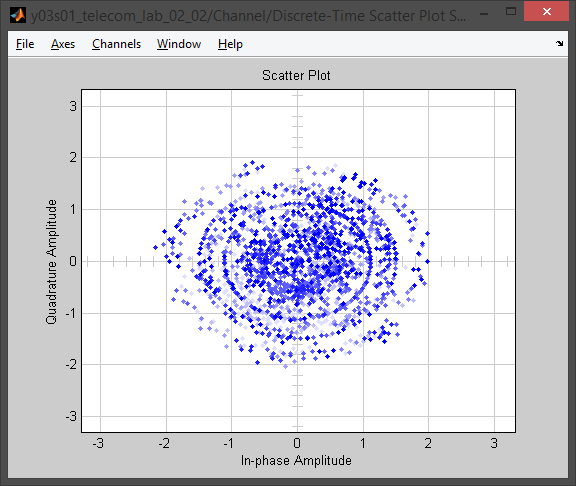
\includegraphics[height = 7\baselineskip]{../01-solution/02-freqshift-1000-hz-channel-scatter-plot.png}
						\caption{}
						\label{subfig:freqshift-signal-trajectory-out}
					\end{subfigure}%
					\begin{subfigure}{\textwidth / 3}
						\centering
						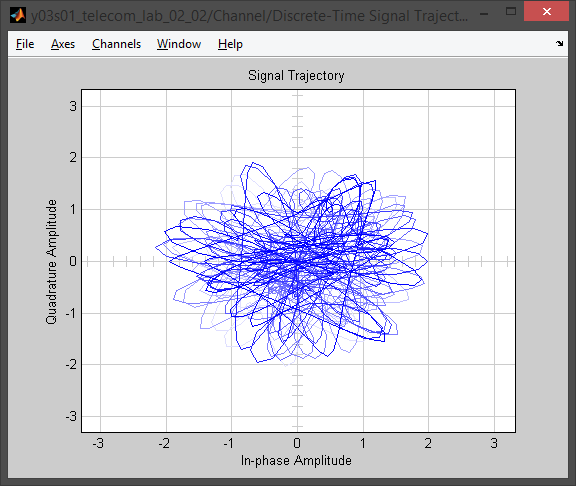
\includegraphics[height = 7\baselineskip]{../01-solution/02-freqshift-1000-hz-channel-signal-trajectory.png}
						\caption{}
						\label{subfig:freqshift-scatter-plot-out}
					\end{subfigure}%
					\caption{Вплив частотної неузгодженості на сигнал: \subref{subfig:freqshift-eye-in}–\subref{subfig:freqshift-scatter-plot-in}~— при значенні~\SI{0}{\hertz}; \subref{subfig:freqshift-eye-out}–\subref{subfig:freqshift-scatter-plot-out}~— при значенні~\SI{1000}{\hertz}}
					\label{fig:freqshift-plots}
				\end{figure}

			\subsubsection{Дробова затримка~\SI{0}{\second}, \SI{3}{\second}}
				Встановлюємо дробову затримку~\SI{0}{\second}, \SI{3}{\second} та~запускаємо моделювання, отримаємо результати на~графіках~(рис.~\ref{fig:fracdelay-spectrum-scope}, \ref{fig:fracdelay-scope}, \ref{fig:fracdelay-plots}).

				\begin{figure}[!htbp]
					\begin{minipage}[t]{0.5\textwidth - 0.5em}
						\centering
						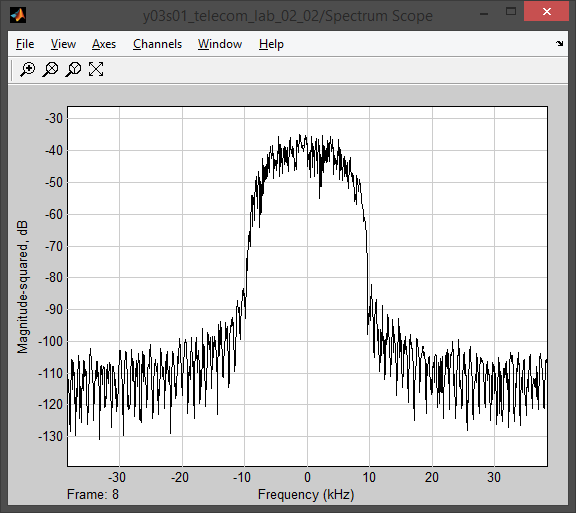
\includegraphics[height = 8\baselineskip]{../01-solution/00-SNR-100db-noshift-modulator-spectrum.png}
						\caption{Спектр сигналу при дробовій затримці \SI{0}{\second}}
						\label{fig:fracdelay-spectrum-scope}
					\end{minipage}\hspace{1em}%
					\begin{minipage}[t]{0.5\textwidth - 0.5em}
						\centering
						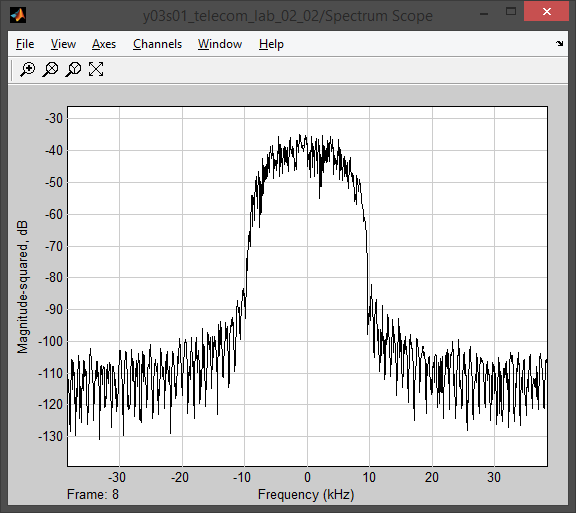
\includegraphics[height = 8\baselineskip]{../01-solution/00-SNR-100db-noshift-modulator-spectrum.png}
						\caption{Спектр сигналу при дробовій затримці \SI{3}{\second}}
						\label{fig:fracdelay-scope}
					\end{minipage}%
				\end{figure}

				\begin{figure}[!htbp]
					\centering
					\begin{subfigure}{\textwidth / 3}
						\centering
						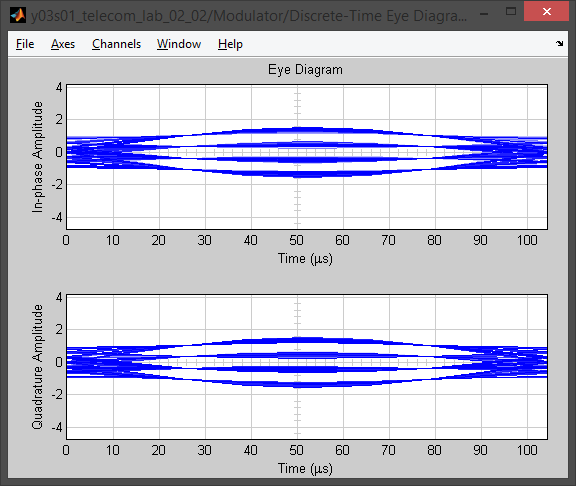
\includegraphics[height = 7\baselineskip]{../01-solution/00-SNR-100db-noshift-modulator-eye-diagram.png}
						\caption{}
						\label{subfig:fracdelay-eye-in}
					\end{subfigure}%
					\begin{subfigure}{\textwidth / 3}
						\centering
						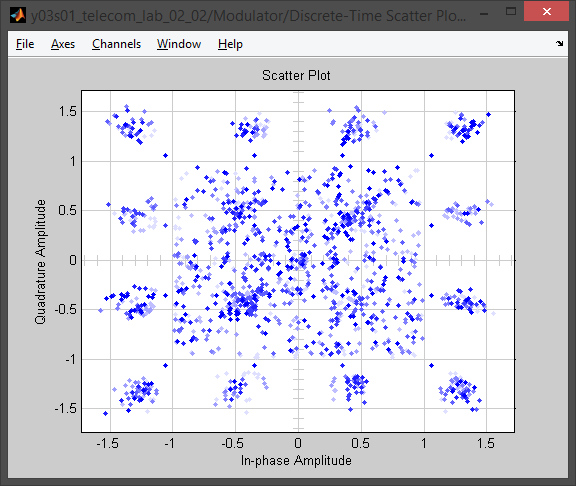
\includegraphics[height = 7\baselineskip]{../01-solution/00-SNR-100db-noshift-modulator-scatter-plot.png}
						\caption{}
						\label{subfig:fracdelay-signal-trajectory-in}
					\end{subfigure}%
					\begin{subfigure}{\textwidth / 3}
						\centering
						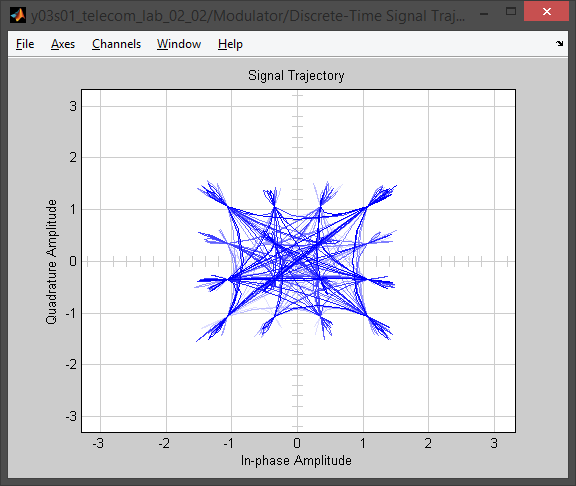
\includegraphics[height = 7\baselineskip]{../01-solution/00-SNR-100db-noshift-modulator-signal-trajectory.png}
						\caption{}
						\label{subfig:fracdelay-scatter-plot-in}
					\end{subfigure}
					\begin{subfigure}{\textwidth / 3}
						\centering
						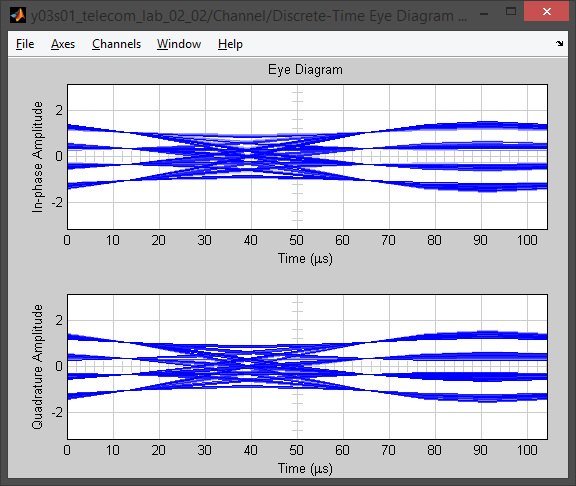
\includegraphics[height = 7\baselineskip]{../01-solution/03-fracdelay-3p0-channel-eye-diagram.png}
						\caption{}
						\label{subfig:fracdelay-eye-out}
					\end{subfigure}%
					\begin{subfigure}{\textwidth / 3}
						\centering
						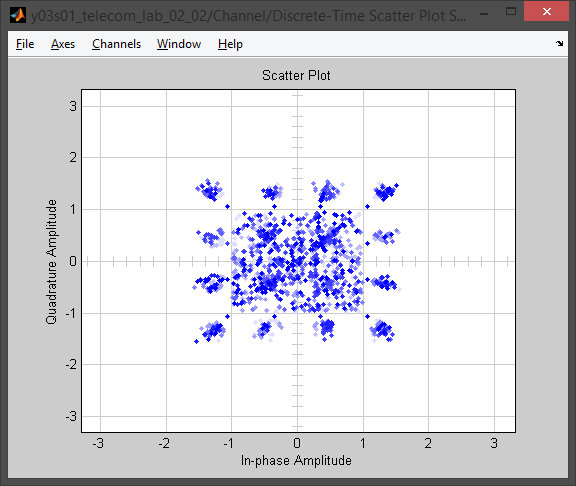
\includegraphics[height = 7\baselineskip]{../01-solution/03-fracdelay-3p0-channel-scatter-plot.png}
						\caption{}
						\label{subfig:fracdelay-signal-trajectory-out}
					\end{subfigure}%
					\begin{subfigure}{\textwidth / 3}
						\centering
						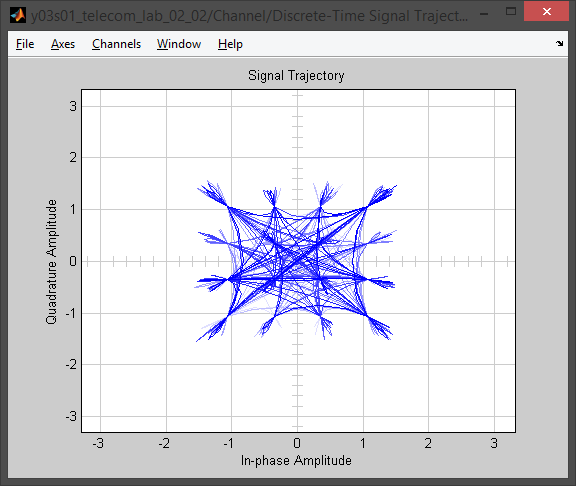
\includegraphics[height = 7\baselineskip]{../01-solution/03-fracdelay-3p0-channel-signal-trajectory.png}
						\caption{}
						\label{subfig:fracdelay-scatter-plot-out}
					\end{subfigure}%
					\caption{Вплив дробової затримки на сигнал: \subref{subfig:fracdelay-eye-in}–\subref{subfig:fracdelay-scatter-plot-in}~— при значенні~\SI{0}{\second}; \subref{subfig:fracdelay-eye-out}–\subref{subfig:fracdelay-scatter-plot-out}~— при значенні~\SI{3}{\second}}
					\label{fig:fracdelay-plots}
				\end{figure}

	\section{Висновок}
		Виконуючи дану лабораторну роботу, ми дослідили явища, що виникають в каналі зв'язку системи передачі цифрової інформації та дослідили вплив відношення «Сигнал — шум», фазового зсуву, частотного зсуву та дробової затримки на сигнал.

\end{document}
